\clearpage
\item \subquestionpoints{5} \textbf{Coding problem.}
The following three problems will deal with a dataset which we have provided in
the following files:
%
\begin{center}
  \url{data/ds3_{train,valid,test}.csv}
\end{center}
%
Each file contains the following columns: $x_1$, $x_2$, $y$, and $t$. As in
Problem 1, there is one example per row.

First we will consider the ideal case, where we have access to the true
$t$-labels for training. In \texttt{src/p02cde\_posonly}, write a logistic
regression classifier that uses $x_1$ and $x_2$ as input features, and train it
using the $t$-labels (you can ignore the $y$-labels for this part). Output the
trained model's predictions on the test set to the file specified in the code.

\ifnum\solutions=1 {
  \begin{answer}
\newline
  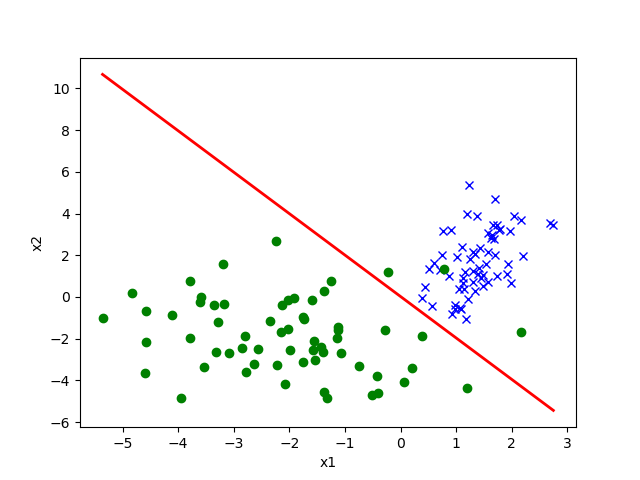
\includegraphics[height=10cm]{C:/Users/feroc/OneDrive/Notability/CS229 Machine Learning/problem_sets/ps1/src/output/p02c_pred.png}
\end{answer}

} \fi
